\chapter{Aplicación TapeYty}
\label{solucionpropuesta}
\ifpdf
  \graphicspath{{Chapter6/Chapter6Figs/PNG/}{Chapter6/Chapter6Figs/PDF/}{Chapter6/Chapter6Figs/}}
\else
  \graphicspath{{Chapter6/Chapter6Figs/EPS/}{Chapter6/Chapter6Figs/}}
\fi

\markboth{\hfill \thechapter. Aplicación \textit{TapeYty}}{\hfill \thechapter. Aplicación \textit{TapeYty}}

En la actualidad, la DSU no cuenta con un \textit{software} que apoye a la toma de decisiones en lo que respecta a la gestión de residuos sólidos urbanos, más específicamente en el área de recolección. Por lo tanto, se propone la implementación de una herramienta GIS que contribuya con la elección de mejores caminos a seguir por los vehículos recolectores, y de esta manera generar mayores beneficios en cuanto a tiempo y distancia, además de garantizar que el servicio sea brindado a todos los domicilios.
%además de contribuir con el cuidado del medio ambiente.

La implementación consta de los siguientes módulos:
\begin{enumerate}
    \item Seguridad: El sistema comprende un mecanismo de autenticación basada en tokens JWT (\textit{JSON Web Tokens}). Se restringe acceso a la aplicación y a los servicios web REST del servidor no autenticados.
    \item Administración: Comprende la gestión (listar, agregar, editar, eliminar) de usuarios y vehículos.
    \item GIS: Este módulo despliega el mapa con las diferentes capas (zona, calle, departamento, distrito) y permite el manejo de capas, la gestión de calles, generación de rutas, despliegue de resultado de ruta optimizada.
    %(Ver Figura \ref{fig:aplicacionRutas}).
\end{enumerate}

\section{Arquitectura de aplicación}

La Figura \ref{fig:disenhoArquitectura} muestra el diseño de la arquitectura de \textit{software} alrededor de la aplicación solución \textit{TapeYty}. Este diseño se divide en dos partes que se explicarán en detalle a continuación.

\begin{figure}[bp]
\centerline{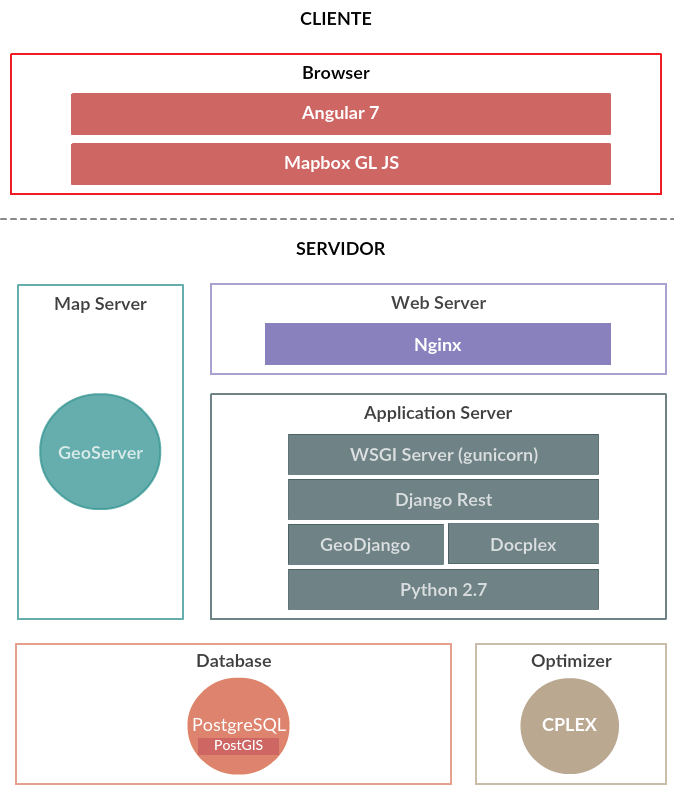
\includegraphics[width=\textwidth]{20190424_WebAppArchitectureDesign.png}}
\caption{Diseño de arquitectura de \textit{TapeYty}.}
\label{fig:disenhoArquitectura}
\end{figure}

\subsection{Cliente}

Desde una computadora portátil o un teléfono móvil el usuario puede acceder a la aplicación e ingresar con sus credenciales desde el navegador (\textit{browser}). Se ejecuta en el navegador el código Javascript generado a partir del código fuente construido con el marco (\textit{framework}) Angular (en su versión 7.0). Angular es un \textit{framework} ampliamente utilizado para el desarrollo de aplicaciones web con excelentes prestaciones en cuanto a rendimiento, escalabilidad, velocidad de respuesta y no menos importante una comunidad numerosa y activa. 

Una de las librerías incorporadas al proyecto cliente (\textit{frontend}) más relevantes es Mapbox GL JS, la cual ofrece funcionalidades relacionadas a mapas, teniendo como gran atractivo su buen desempeño durante el tiempo de renderizado de los mapas y datos geográficos.
% Utiliza WebGL, es una especificacion estandar que define una API javascript para la renderizacion de graficos en 3D dentro de cualquier navegador web. Aprovecha mejor la GPU(Unidad de procesamiento gráfico) desde cualquier navegador (web) que soporte OpenGL 2.0 o mayor.

\subsection{Servidor}

El lado servidor presenta mayor complejidad ya que concentra varios componentes que además deben interactuar unos con otros.

Como parte de la solución, se utiliza el gestor de base de datos relacional PostgreSQL (versión 10.8) con su extensión PostGIS (version 2.4), donde están almacenadas las distintas informaciones obtenidas, geográficas o no, excepto los datos (\textit{shapes}) que provienen del SNC de Paraguay.

Los mapas bases de Departamentos y Distritos del SNC son almacenados en el servidor de mapas Geoserver que se muestra en la Figura \ref{fig:disenhoArquitectura}. También se crea una conexión con la base de datos para poner a disposición las capas o mapas de calles y zonas, en modo lectura, donde el servidor ofrece servicios web de mapas TMS (\textit{Tile Map Service}), servicio que maneja estrategias de caché de cuadros de imágenes para mostrar los mapas con mayor velocidad dando un mejor rendimiento a la aplicación.

% El servidor de mapas GeoServer consiste en un servidor de código abierto escrito en Java que permite a los usuarios compartir y editar datos espaciales. En este servidor se almacenan los mapas bases de Departamentos y Distritos del Catastro Nacional. Además, se crea una conexión con la base de datos para poner a disposición las capas o mapas de calles y zonas, en modo lectura, donde el servidor ofrece servicios web de mapas como por ejemplo \textit{TMS} (\textit{Tile Map Service}), servicio que maneja estrategias de caché de cuadros de imágenes para mostrar los mapas con mayor velocidad dando un mejor rendimiento a la aplicación.

Para resolver el modelo matemático seleccionado se requiere de un \textit{software} especializado para ello. Se opta por la herramienta \textit{CPLEX Optimizer} de IBM \citep{CPLEXOptimizer} en su versión académica 12.8, ya utilizado en trabajos previos \citep{Vecchi2016ACollection,Ramos2018TheApproaches,BabaeeTirkolaee2019DevelopingStudy}. El modelo matemático puede ser codificado en CPLEX con el lenguaje OPL ({\textit{Optimization Programming Language}}), provee además interfaces C, C++, Java y Python para su modelado. Sin embargo, estas interfaces no son usadas directamente para modelar sino a través de la librería Docplex \citep{Docplex} detallada más adelante.

Para el desarrollo propio de una aplicación web una de las preocupaciones más importantes es la elección del lenguaje y el \textit{framework} sobre los cuales estará construida. En este trabajo se opta por el lenguaje Python, conjuntamente con el \textit{framework} GIS GeoDjango. En el área GIS, Python es uno de los lenguajes más utilizados a lo largo del tiempo, pudiéndose encontrar muchas funciones, librerías, \textit{software}, entre otros; escritos con este lenguaje. GeoDjango, basado en Django, tiene la virtud de ser robusto, provee un modelo de programación Modelo-Vista-Controlador MVC (\textit{Model-View-Controller}) y facilita el desarrollo de aplicaciones Web.

La librería Docplex de Python resulta en una sencilla integración con el \textit{framework}, también permite formular el modelo de forma clara y directa en comparación con las interfaces de CPLEX, resultando muy similar a la formulación con el lenguaje OPL (Ver Algoritmo \ref{codigoDocplex}).

\hfill
\begin{lstlisting}[language=Python,caption={Fragmento de código en Docplex},label={codigoDocplex}]
from docplex.mp.model import Model

# ************************ INSTANCIA DEL MODELO ******************************

moron_model = Model(name='moron')
    
# ************************* VARIABLES DE DECISION ****************************

s = {i: moron_model.binary_var(name='s_{0}_{1}'.
    format(i.gis_nodo.gis_nodo_id, i.nodo_expandido_id)) 
    for i in iniciales}
t = {t: moron_model.binary_var(name='t_{0}_{1}'.
    format(t.gis_nodo.gis_nodo_id, t.nodo_expandido_id)) 
    for t in nodos_expandidos}

# **************************FUNCION OBJETIVO *********************************
moron_model.minimize(
    moron_model.sum(x[a.nodo_expandido_origen, a.nodo_expandido_destino] * a.peso 
    for a in arcos_expandidos))
    
# **************************** RESTRICCIONES *********************************
# Garantizan que el nodo inicial sea unico
moron_model.add_constraint(moron_model.sum(s[i] for i in iniciales) == 1)

# Garantizan que el nodo final sea unico
moron_model.add_constraint(moron_model.sum(t[i] for i in nodos_expandidos) == 1))
\end{lstlisting}

Con Docplex y GeoDjango se implementa toda la lógica de negocio de la aplicación. Para poder acceder a esta lógica desde el cliente se brinda una API (\textit{Application Programming Interface}). Para ello, se utiliza el protocolo de comunicación de intercambio de datos RESTful con la librería Django REST Framework y Django Rest Framework GIS. Se implementan los servicios para los módulos citados anteriormente como: agregar, eliminar y editar usuarios, editar propiedades alfanuméricas de calles, generar la ruta óptima de una zona, entre muchos otros; con estructuras de datos en formato JSON (\textit{JavaScript Object Notation}) y geoJSON.

Con ésto la aplicación está prácticamente lista, queda preparar el ambiente de producción para su implantación. Se instala uno de los servidores web más comunes actualmente, Nginx. El servidor web recibe una solicitud HTTP del cliente (el navegador), interpreta la solicitud y la envía a la puerta de enlace (\textit{gateway}). El \textit{gateway} Gunicorn es un servidor HTTP de Interfaz de Pasarela del Servidor Web de Python (WSGI, \textit{Web Server Gateway Interface}) que traduce la solicitud recibida del servidor web para que la aplicación pueda manejarlo. Y por último se tiene la aplicación servidor que a través de su API Rest recibe la petición para luego procesar y responder.

\section{Aplicación}

En esta sección se detalla las principales funcionalidades que constituyen la aplicación \textit{TapeYty}. En el Apéndice \ref{sec:manual-usuario} se encuentra disponible el manual de usuario donde se detalla la totalidad de las funcionalidades del sistema.

\subsection{Modelo de datos}

La Figura \ref{fig:DERTapeYty} muestra el modelado de datos a partir de un Diagrama Entidad-Relación (DER), diseñado con la herramienta SQLPowerArchitect \citep{SQLArchitect} en su versión 1.0.8. A continuación, en la Tabla \ref{tab:descripcionDER} se detalla brevemente cada tabla en el DER.

\begin{landscape}
\begin{figure*}[tbp]
\centerline{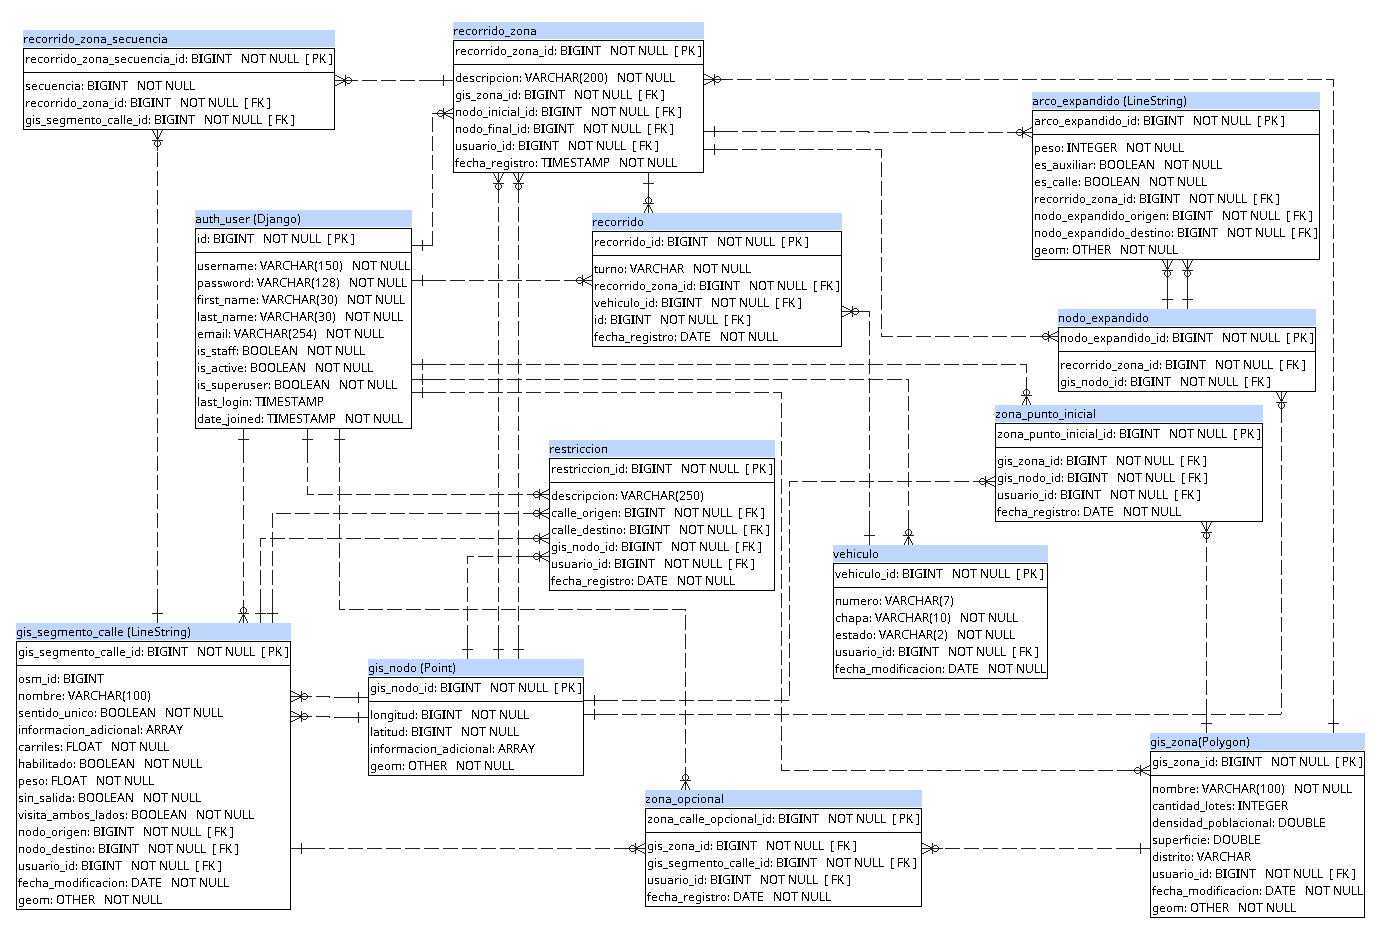
\includegraphics[height=\textheight]{20190716_DER.png}}
\caption{Diagrama Entidad-Relación de \textit{TapeYty}.}
\label{fig:DERTapeYty}
\end{figure*}
\end{landscape}

% Please add the following required packages to your document preamble:
% \usepackage{multirow}
% \usepackage{graphicx}
\begin{table}[]
\caption{Descripción del modelo de datos de \textit{TapeYty}.}
\label{tab:descripcionDER}
\resizebox{\textwidth}{!}{%
\begin{tabular}{lll}
\hline
Uso                                                                                              & Nombre de tabla            & Descripción                                                                                                                                                        \\ \hline
\begin{tabular}[c]{@{}l@{}}Autenticación y \\ auditoría\end{tabular}                             & auth\_user                 & \begin{tabular}[c]{@{}l@{}}Creada por Django, es referenciada en todas las tablas que \\ pueden ser editadas por el usuario en la aplicación \textit{TapeYty}.\end{tabular} \\ \hline
\multirow{3}{*}{Capas}                                                                           & gis\_nodo                  & \begin{tabular}[c]{@{}l@{}}Representan puntos en el mapa. Los datos iniciales son \\ cargados desde OSM.\end{tabular}                                              \\
                                                                                                 & gis\_segmento\_calle       & \begin{tabular}[c]{@{}l@{}}Representan segmentos de calle en el mapa. Los datos \\ iniciales son cargados desde OSM.\end{tabular}                                  \\
                                                                                                 & gis\_zona                  & \begin{tabular}[c]{@{}l@{}}Representan las zonas de trabajo del departamento de\\ recolección de la DSU.\end{tabular}                                              \\ \hline
\multirow{3}{*}{\begin{tabular}[c]{@{}l@{}}Lógica de recolección\\ DSU\end{tabular}}             & zona\_calle\_opcional      & \begin{tabular}[c]{@{}l@{}}Representan las calles dentro o en el límite de una zona \\ que pueden no ser recorridos por el vehículo recolector.\end{tabular}       \\
                                                                                                 & zona\_punto\_incial        & \begin{tabular}[c]{@{}l@{}}Representan puntos en el límite de una zona en donde \\ se puede empezar el recorrido.\end{tabular}                                    \\
                                                                                                 & restricción                & Representan prohibiciones de giro y contramano.                                                                                                                    \\ \hline
\multirow{2}{*}{\begin{tabular}[c]{@{}l@{}}Representación del \\ grafo $G'$\end{tabular}} & nodo\_expandido            & Representa el conjunto $V$ del modelado.                                                                                                                             \\
                                                                                                 & arco\_expandido            & Representa el conjunto $A$ del modelado.                                                                                                                             \\ \hline
\multirow{4}{*}{Recorrido}                                                                       & vehículo                   & Representa un vehículo de la DSU.                                                                                                                                  \\
                                                                                                 & recorrido                  & El recorrido es asociado a un vehículo y turno de la DSU.                                                                                                          \\
                                                                                                 & recorrido\_zona            & Cada recorrido es asociado a una zona.                                                                                                                             \\
                                                                                                 & recorrido\_zona\_secuencia & Representa la secuencia de un recorrido en una zona.                                                                                                               \\ \hline
\end{tabular}%
}
\end{table}

\subsection{Funcionalidades más relevantes}

\subsubsection{Editar un segmento de calle}

El sistema permite modificar propiedades (no geométricas) de los segmentos de calles. En la Figura \ref{fig:edicionCalles} se selecciona un segmento de la calle General Bernardino Caballero indicado con un color amarillo y con sus puntos extremos pintados.

En el panel derecho de la aplicación se muestra el sentido del segmento, el punto de color rosa claro representa en el mapa el origen del trayecto a seguir mientras que el punto lila indica su destino. Además, se observa que el segmento de calle se encuentra habilitado para su circulación. El usuario puede modificar el sentido del segmento invirtiendo el origen y destino, convertir el segmento a uno de doble sentido y deshabilitar el segmento de calle para su circulación. os segmentos de calles deshabilitados no forman parte de las rutas generadas.
 
Es importante mencionar que un cambio en las propiedades de un segmento puede generar inconsistencias en la red de calles, y consecuentemente, produzca un resultado infactible en la generación de la ruta optimizada. Por ejemplo, si un segmento de calle sin salida habilitado se establece como de único sentido, no se podrá acceder o salir del mismo impidiéndose que se cumplan las restricciones de conservación de flujo del modelo.

\begin{figure}[H]
\centerline{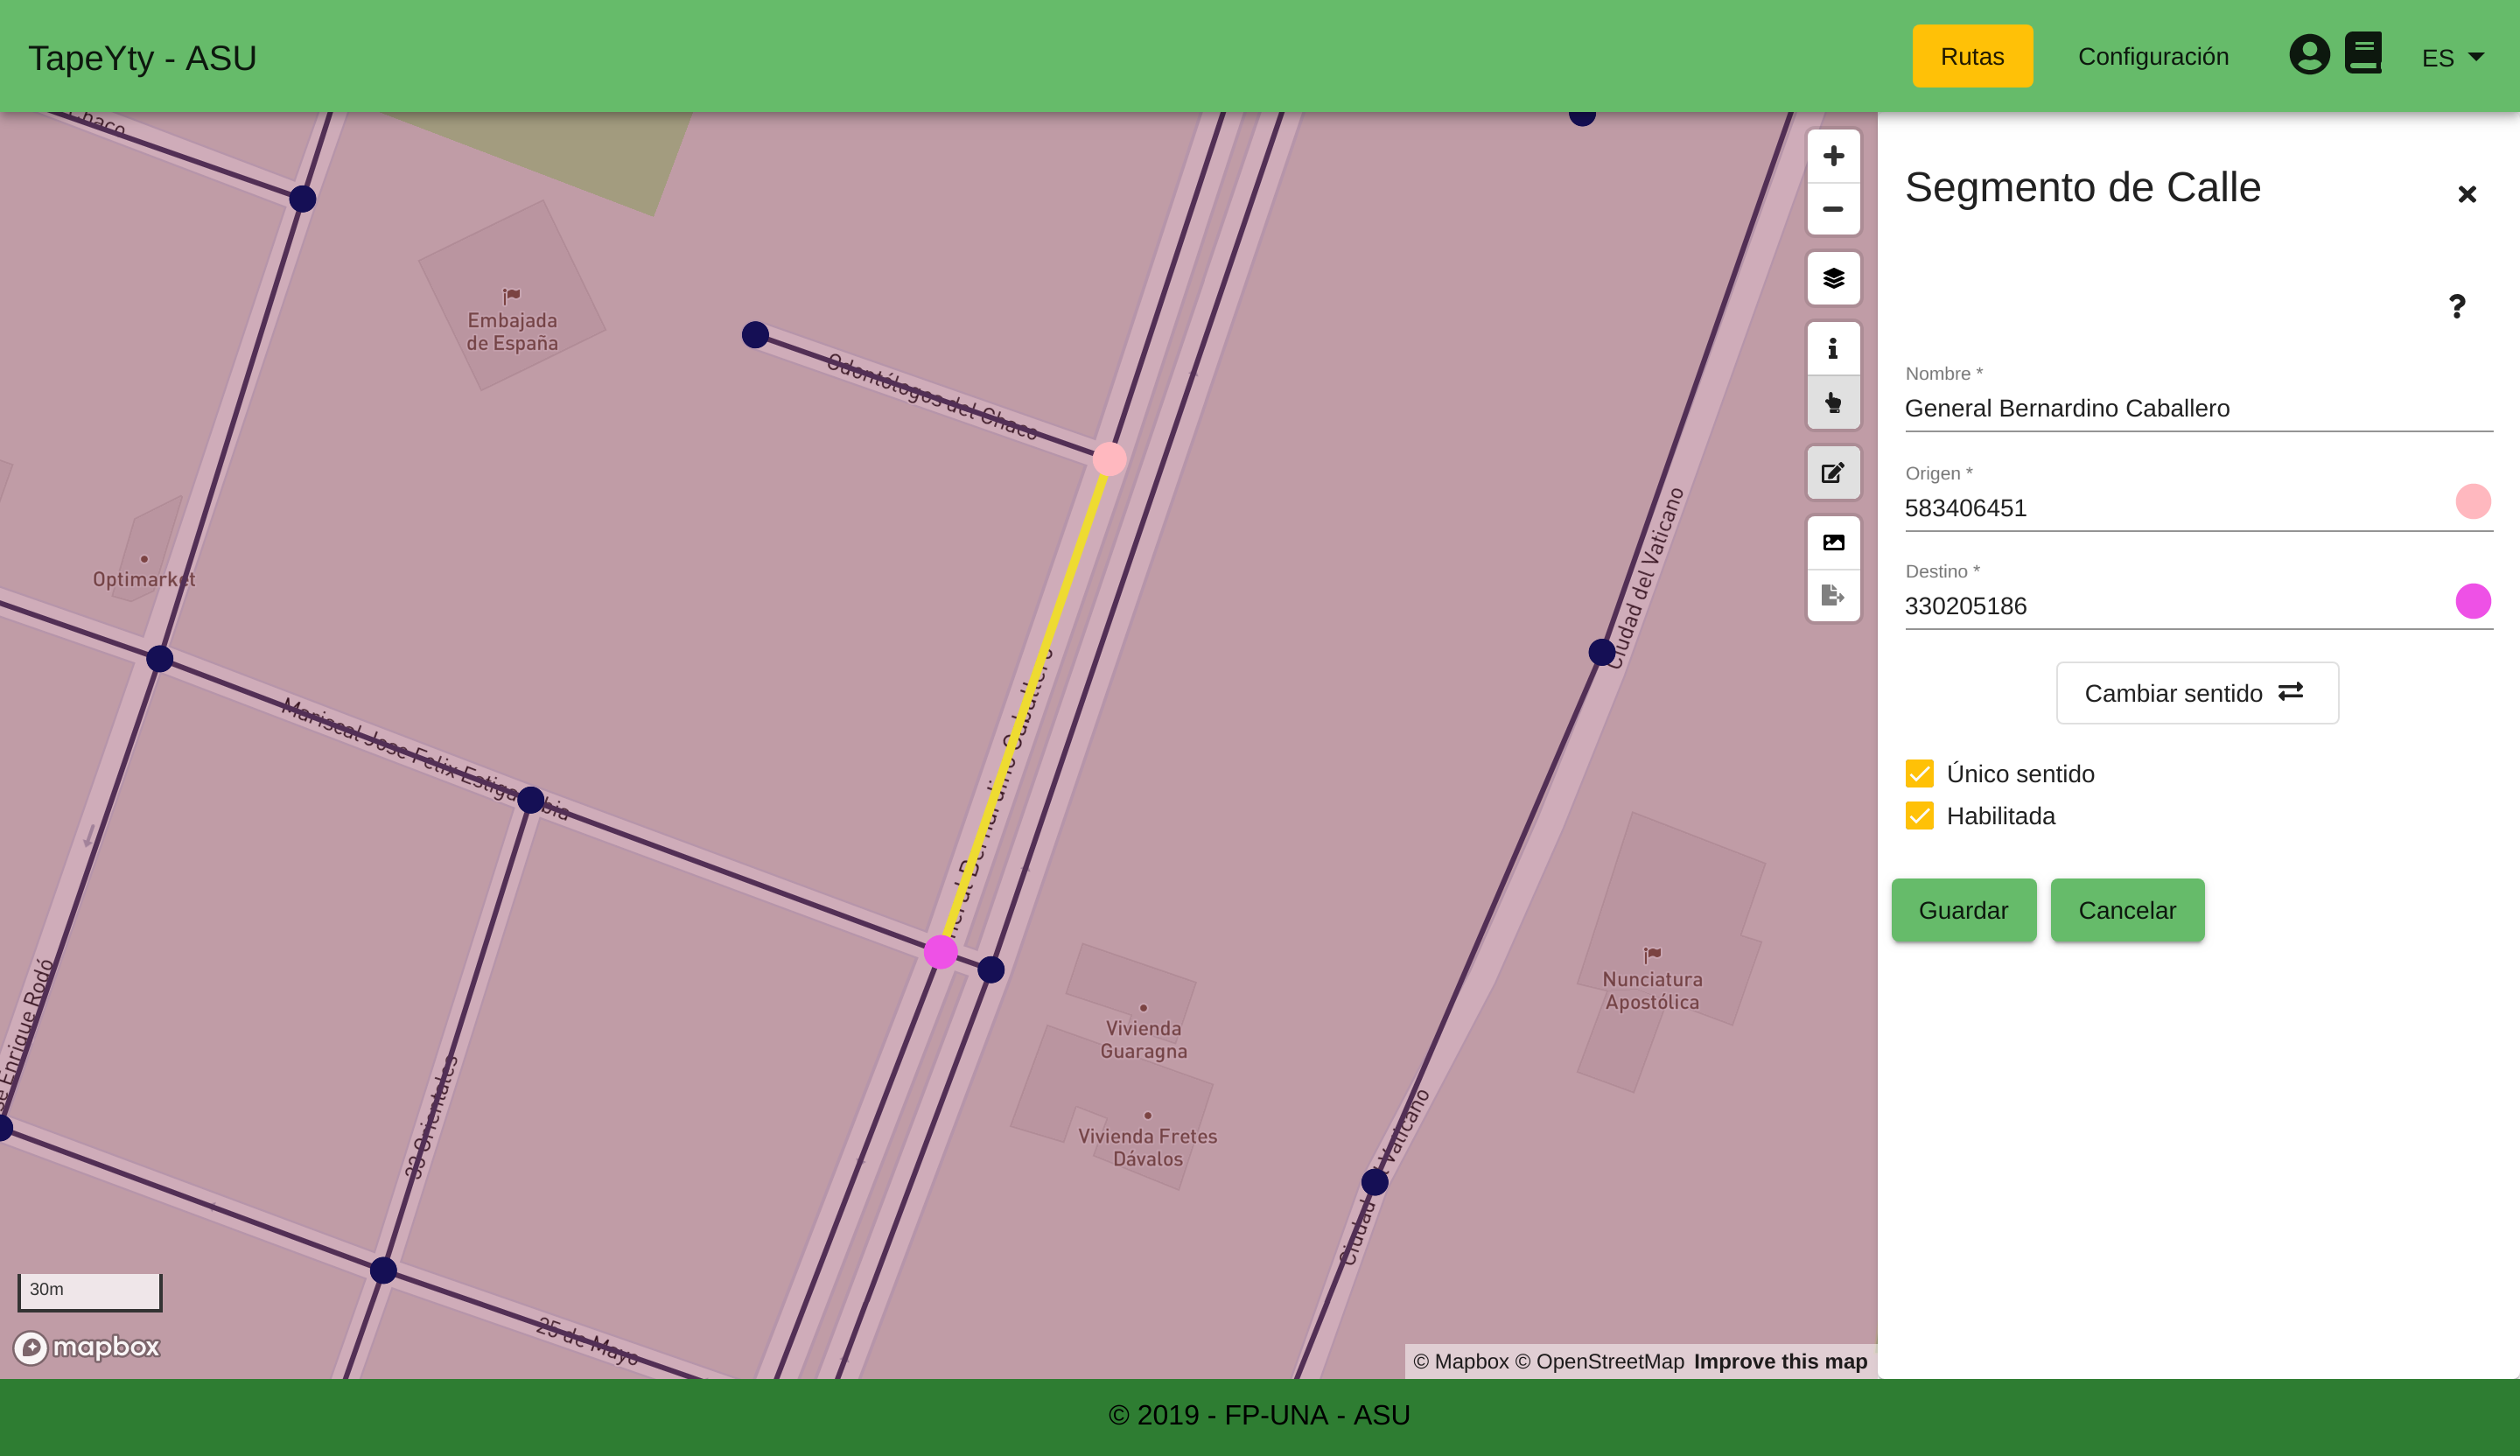
\includegraphics[width=\textwidth]{edicionCalle.png}}
\caption{Edición de un segmento de calle en \textit{TapeYty}.}
\label{fig:edicionCalles}
\end{figure}

\subsubsection{Agregar calles opcionales para el recorrido de una zona}

% Para poder establecer si las calles que se encuentran en el límite de una zona pertenecen o no a la zona en cuestión en el sistema se definen las calles opcionales de una zona. 
En la Figura \ref{fig:callesOpcionales} se observan que los segmentos de las Avenidas Kubitschek, Mariscal López y General Santos que limitan la zona seleccionada se encuentran resaltadas en color verde, indicándose como opcionales, es decir, en el modelo se establece que estos segmentos no requieren ser atravesados para su respectiva recolección.

Una vez que el usuario selecciona la opción de agregar o eliminar los segmentos de calle opcionales de una zona, se despliegan los segmentos de calles que se encuentran cubiertos por la zona seleccionada utilizando la función \textit{coveredby} de Django que es equivalente a la función \textit{ST\_CoveredBy} en PostGIS.

\begin{figure}[H]
\centerline{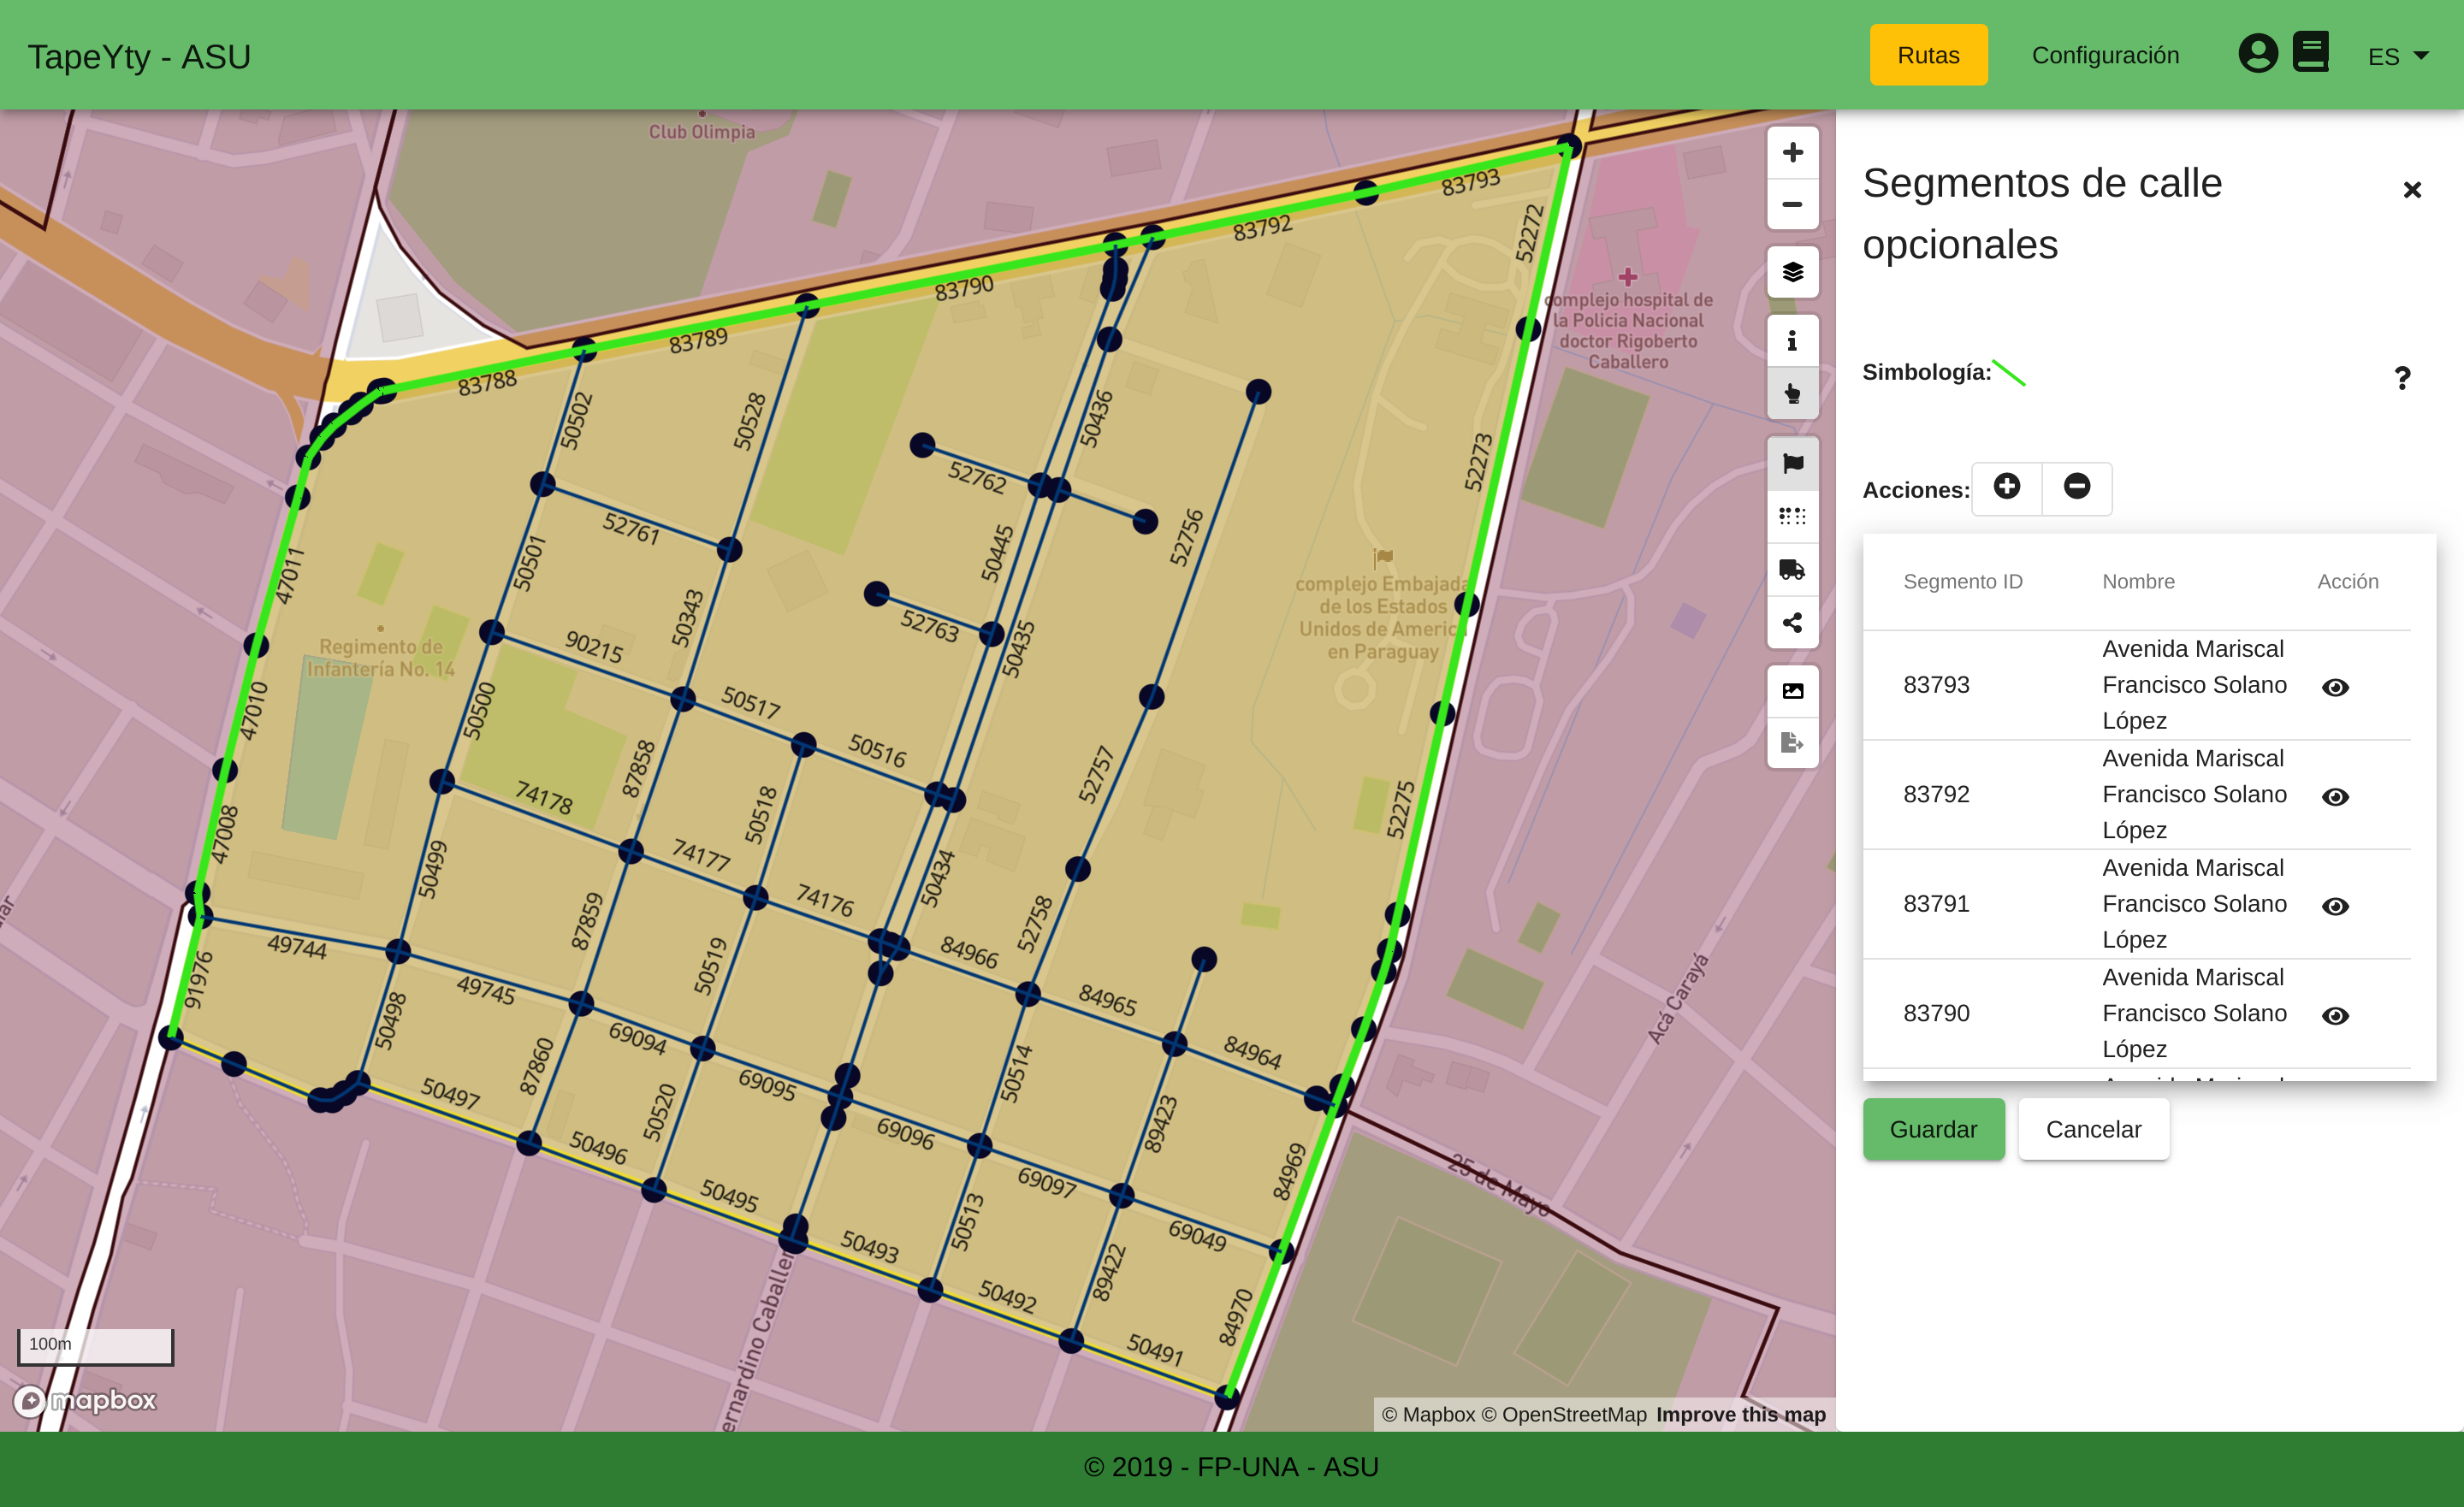
\includegraphics[width=\textwidth]{callesOpcionales.png}}
\caption{Agregar o eliminar calles opcionales de una zona en \textit{TapeYty}.}
\label{fig:callesOpcionales}
\end{figure}

\subsubsection{Agregar posibles puntos iniciales para el recorrido de una zona}

El conductor del camión recolector en el inicio de su recorrido dentro de una zona deberá atravesar primeramente una de las calles que conforman el límite de dicha zona. Los nodos o puntos extremos de los segmentos que forman parte de estos límites, por ende, conforman los posibles puntos iniciales del recorrido y a su vez corresponden a los datos de entrada del modelo. 

En la mayoría de los casos, es probable que el camión ingrese por alguno de los puntos más cercanos de hacia donde viene dirigido el conductor y no precisamente del otro extremo de la zona. Esto deriva en la necesidad de seleccionar no todos, sino más bien unos pocos puntos del borde de la zona como posibles inicio de la ruta óptima.

En la Figura \ref{fig:puntosIniciales} se observa en el mapa en color verde los posibles puntos de inicio para el camino a seguir. En el panel se despliega la lista de dichos puntos y también se tiene la posibilidad de editar la lista, agregando o eliminando puntos.

\begin{figure}[H]
\centerline{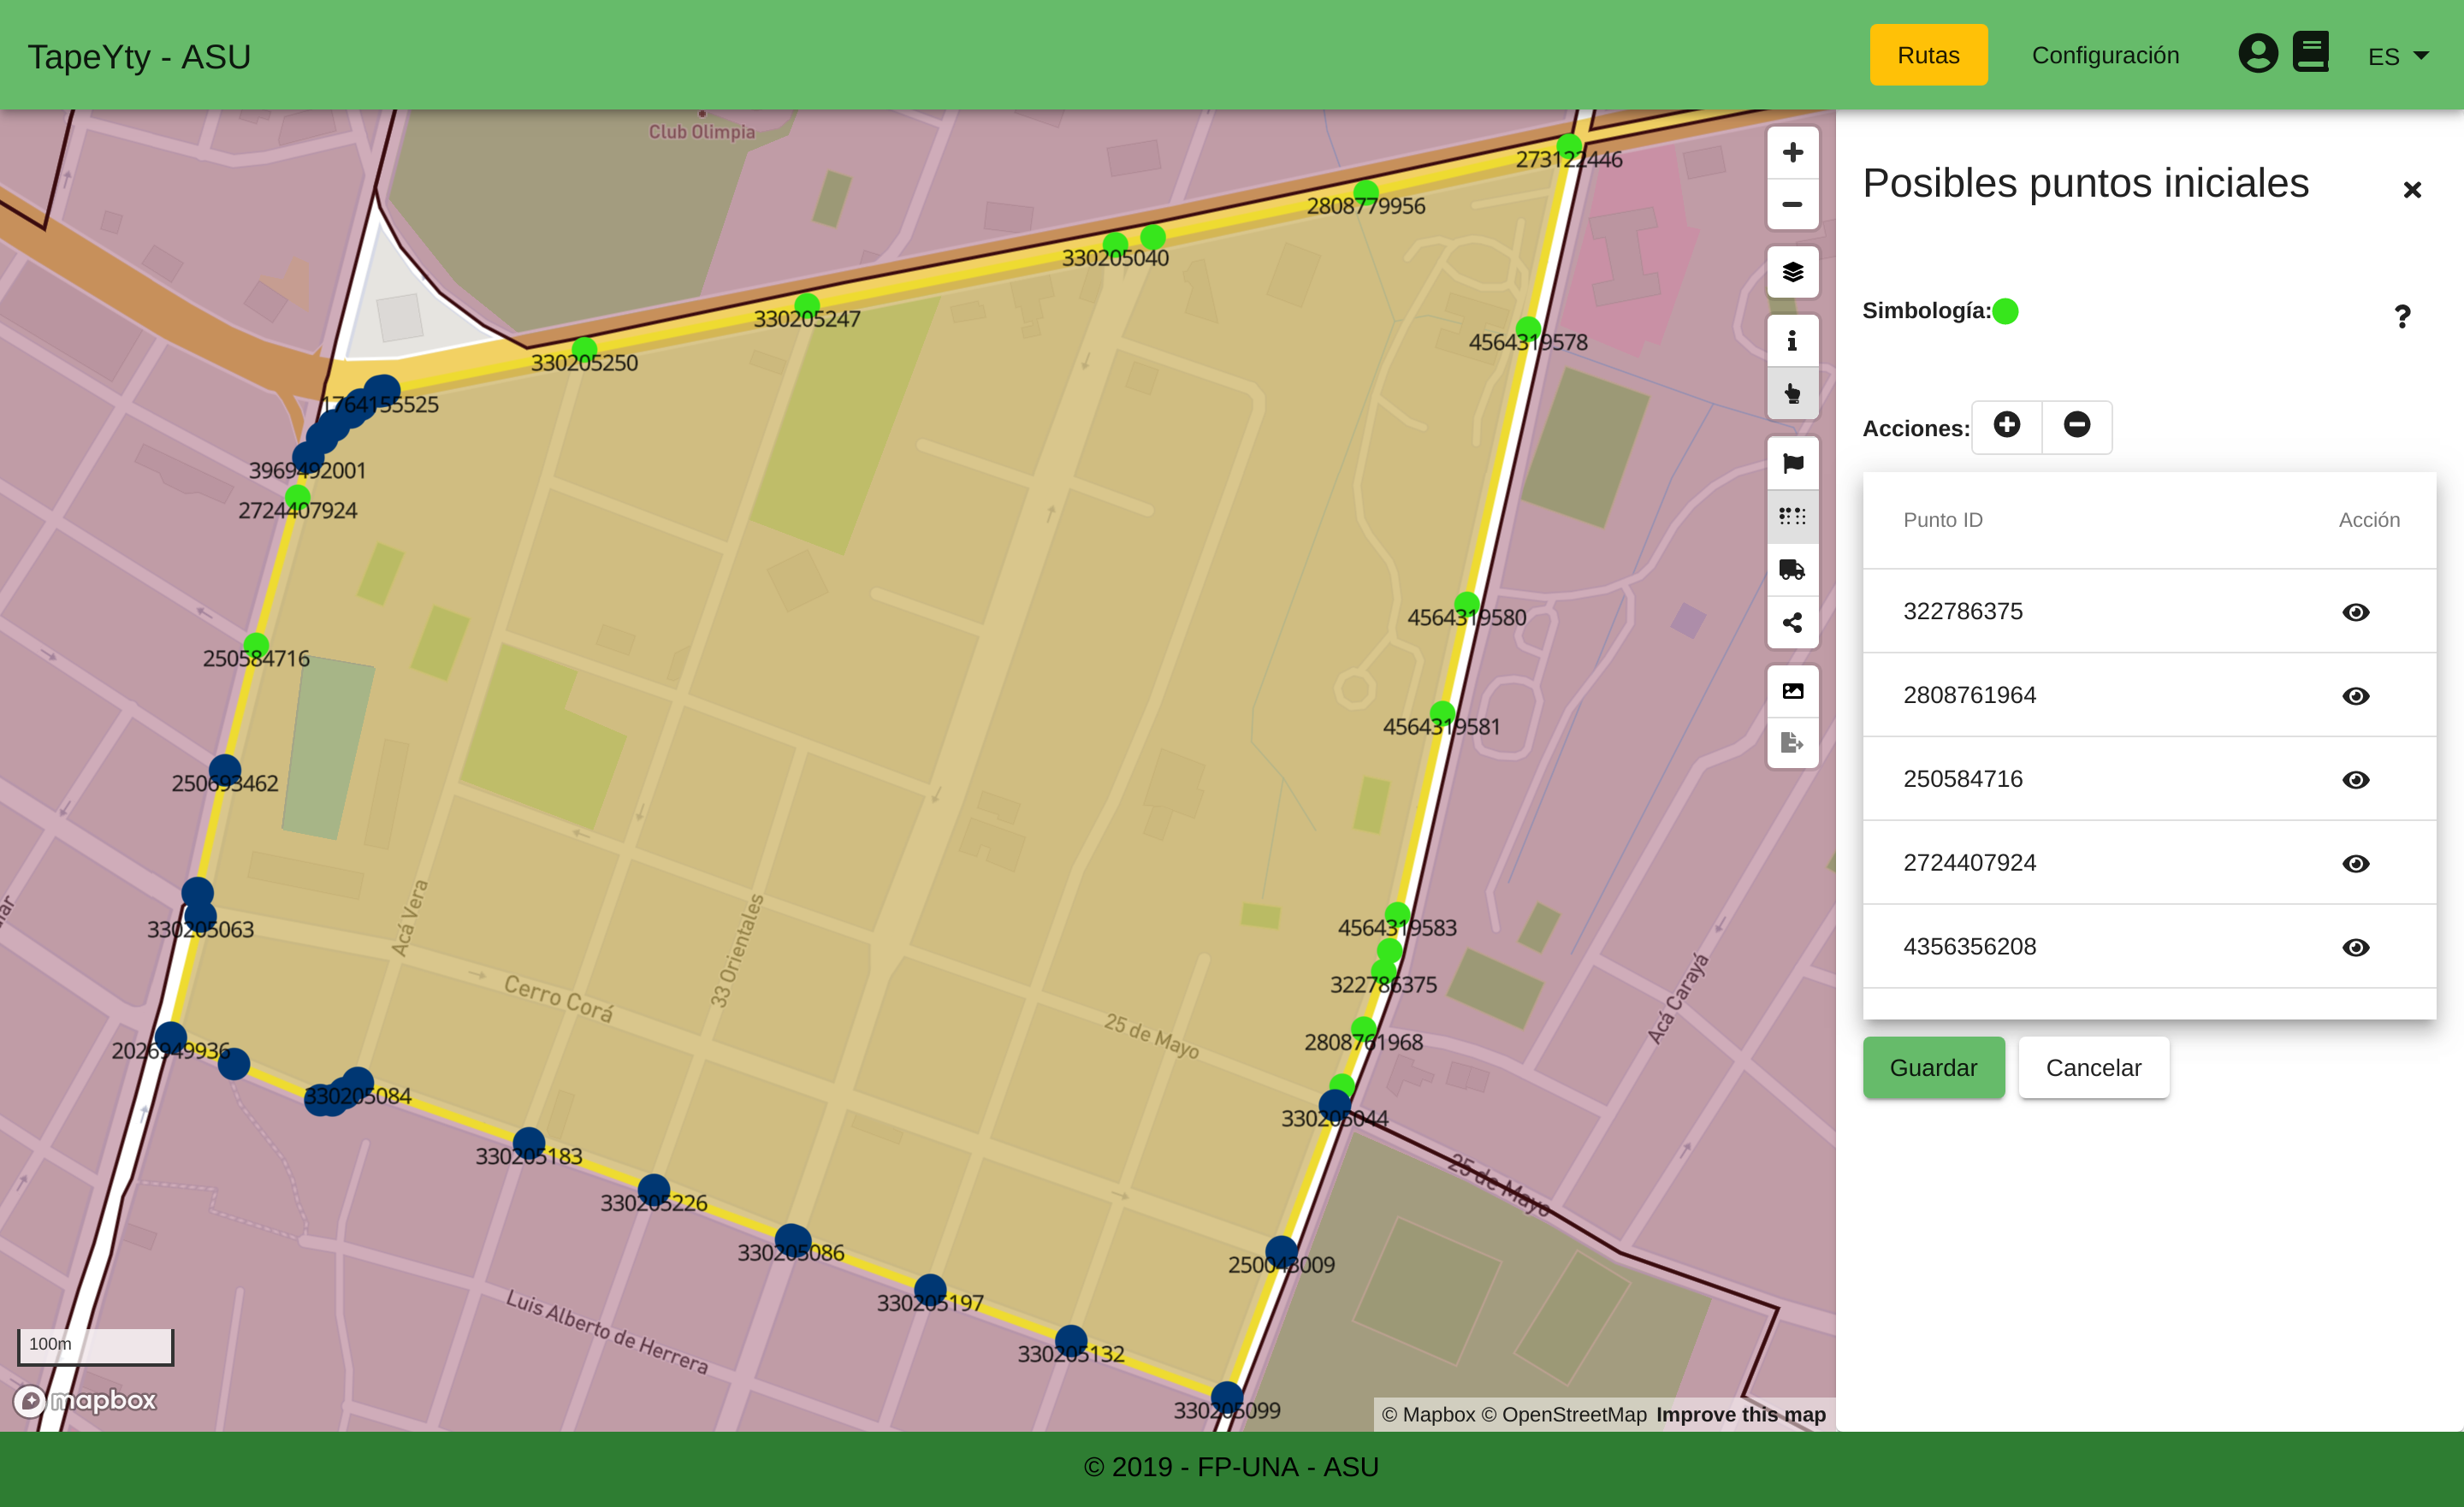
\includegraphics[width=\textwidth]{puntosIniciales.png}}
\caption{Agregar o eliminar posibles puntos de inicio de una zona en \textit{TapeYty}.}
\label{fig:puntosIniciales}
\end{figure}

\subsubsection{Agregar restricciones de red de ruta}

Para poder manejar correctamente las restricciones de la red de calles, el sistema permite agregar y eliminar restricciones que existan entre dos segmentos de calles que tengan un punto en común. 

En la Figura \ref{fig:restriccion} en el panel a la derecha de la aplicación se listan todas las restricciones que se dibujan en el mapa, desde el listado se puede eliminar una restricción o se puede seleccionar. Al seleccionar se resalta la prohibición de giro a la derecha desde la calle 25 de Mayo hacia la calle 33 Orientales.

En el mapa de la Figura \ref{fig:restriccion} se observa en color verde las restricciones que existen sobre los segmentos de calles que pertenecen a la zona seleccionada y además sobre las que se encuentran hasta 220 metros alrededor de la zona en cuestión, ya que para generar la ruta de recolección se tienen en cuenta las calles dentro de una zona como las que se encuentran en una banda perimetral de 220 metros representadas como segmentos opcionales.

\begin{figure}[H]
\centerline{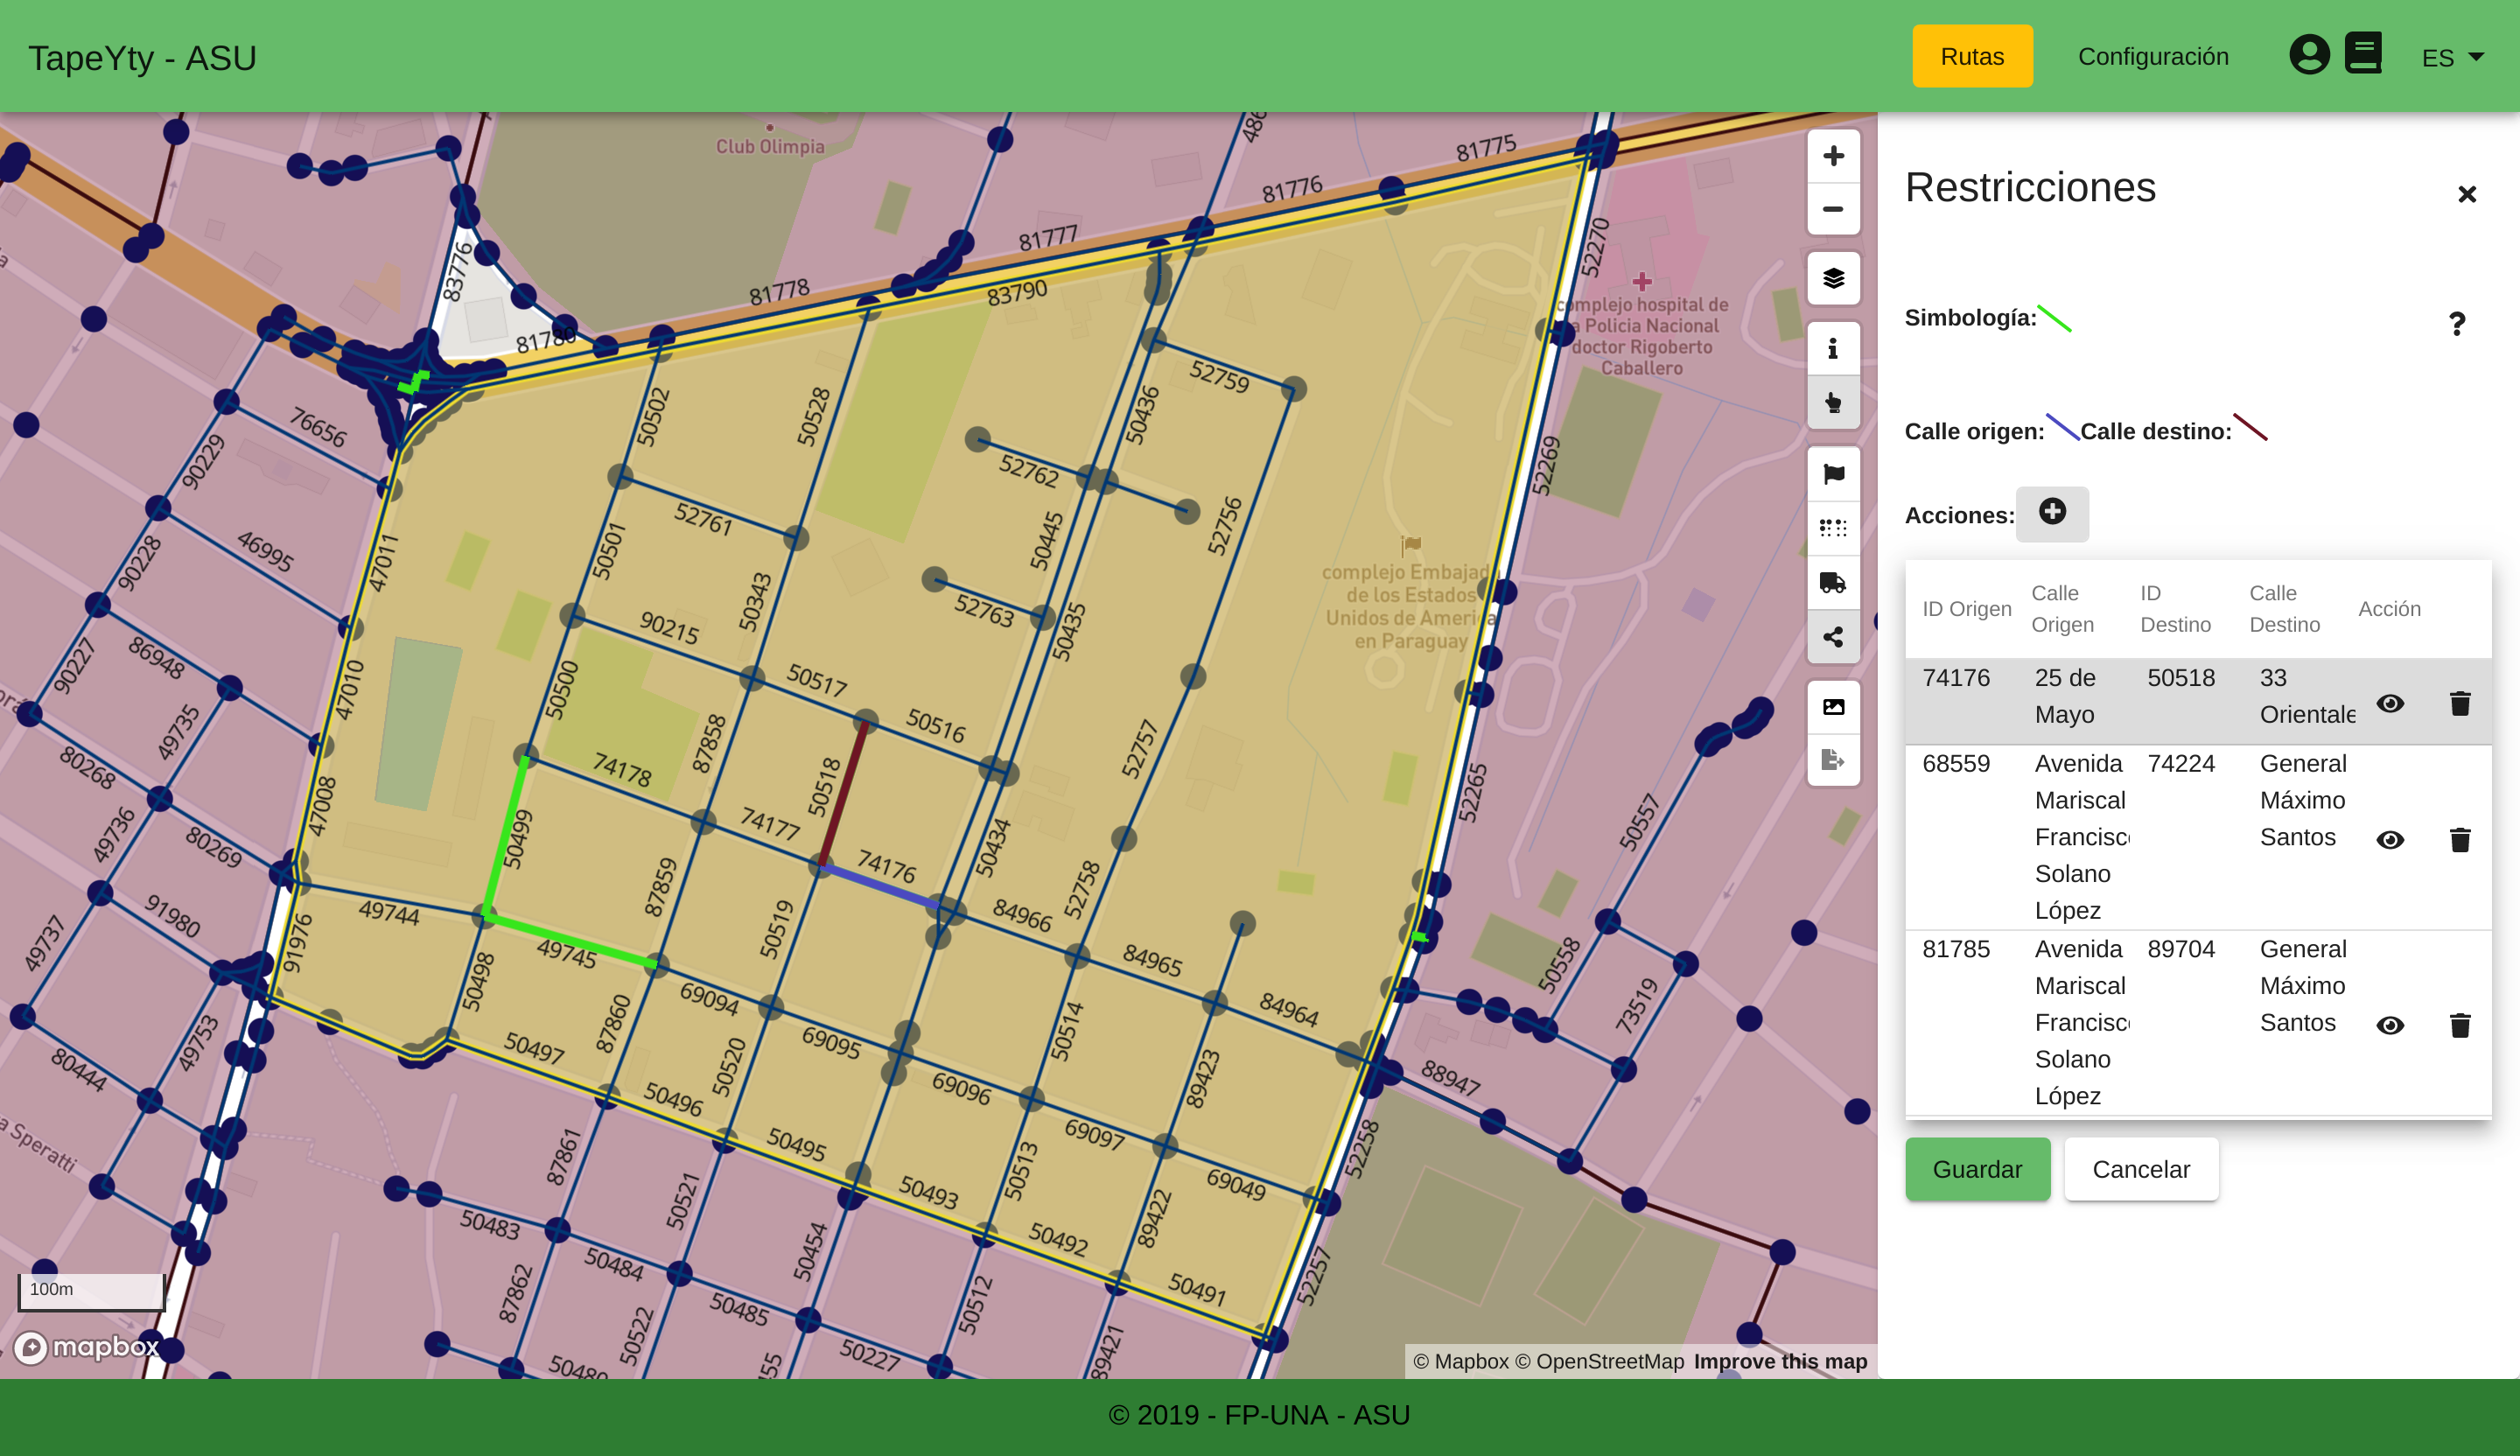
\includegraphics[width=\textwidth]{restricciones.png}}
\caption{Agregar o eliminar restricciones de giro y contramano en \textit{TapeYty}.}
\label{fig:restriccion}
\end{figure}

\subsubsection{Desplegar y descargar la ruta optimizada}

La Figura \ref{fig:generacionRuta} muestra finalmente como se despliega en el mapa la ruta óptima generada por el sistema. Se indican de forma clara los puntos inicial (color verde) y final (color rojo) del recorrido. Los segmentos contienen etiquetas que representan la secuencia en que deben ser visitados cada uno de ellos. Un segmento contiene una etiqueta con valores entre comas en el caso en que se pase más de una vez por el mismo segmento. Algunos valores de secuencia pueden no ser visibles a cierta escala por el simple hecho de evitar la superposición de etiquetas en segmentos contiguos. Para visualizarlos se debe realizar un acercamiento en el mapa desde la aplicación.

Es posible acceder al histórico de recorridos generados en una zona, buscarlos por alguna propiedad como nota o fecha para volver a desplegar uno de ellos en un momento dado. Se brinda además la opción de exportar el resultado y descargarlo como imagen en formato PNG y como archivo en formato GPX. El archivo GPX permite la navegación, por ejemplo, desde cualquier dispositivo GPS o a través de una aplicación del teléfono apropiada para ello como lo es ``Mi Ruta'' \citep{MiRuta}.

\begin{figure}[H]
\centerline{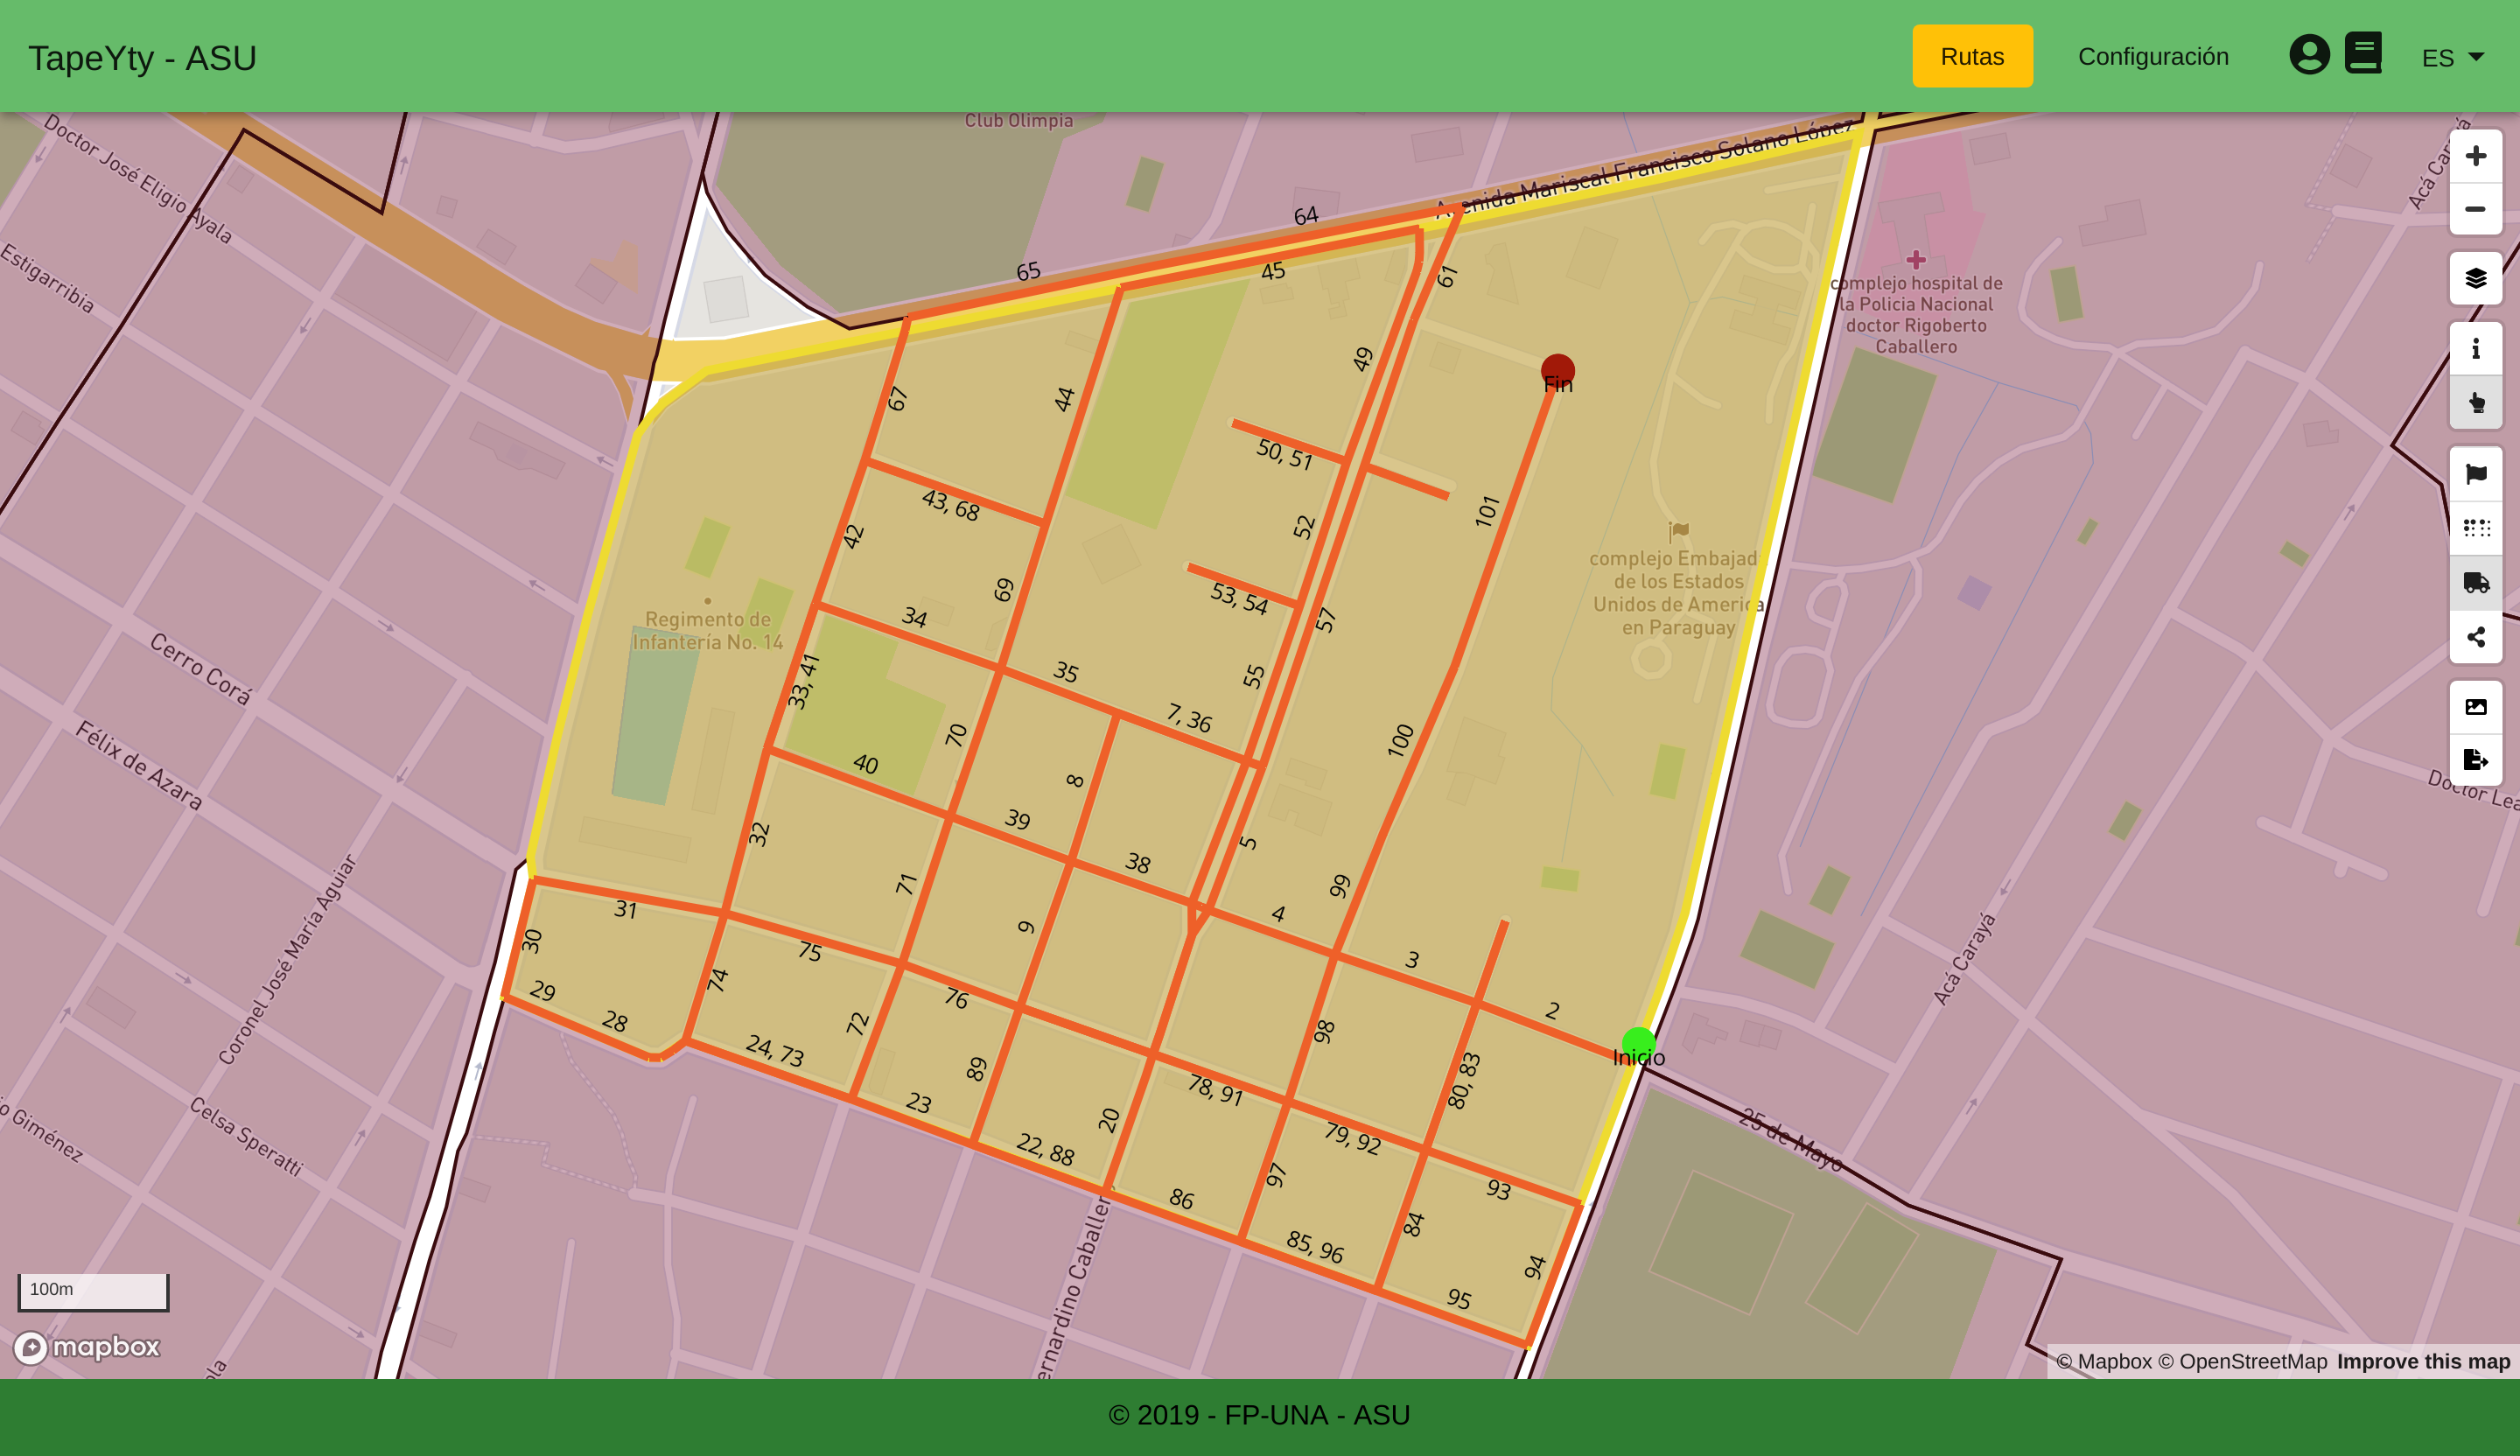
\includegraphics[width=\textwidth]{generacionRuta.png}}
\caption{Despliegue de ruta generada con \textit{TapeYty} en una zona de trabajo.}
\label{fig:generacionRuta}
\end{figure}


% Uno de los parámetros de entrada para el algoritmo, es el conjunto de los posibles puntos o nodos que podrán ser inicio del recorrido. A cada zona, lista de posibles nodos iniciales . Hablar con una imagen de la aplicación de dicha funcionalidad, de que si no se elige ninguno se realiza X operación GIS(ver Figura NN).

